\chapter{Results}
\label{capitolo5}


\begin{quotation}
{\footnotesize
\noindent \emph{``Terence: Ma scusa di che ti preoccupi, i piedipiatti hanno altro a cui pensare, in questo momento stanno cercando due cadaveri scomparsi \\
Bud: Se non spegni quella sirena uno di quei due cadaveri scomparsi lo trovano di sicuro!''}
\begin{flushright}
Nati con la camicia
\end{flushright}
}
\end{quotation}
\vspace{0.5cm}

\noindent A comparison of the simulation with respect to the software OASYS developed by Manuel Sanchez Del Rio and with a paper \cite{resta2015nested} in order to demonstrate the correct operation of the program. The comparison with OASYS check the work of all the component apart from Montel system (mirrors, lens, KB ...), the paper is dedicate for the Montel system, because this particular kind of optical system is not implemented on OASYS.

\section{Testing with OASYS}

\section{Testing with the paper}
The system simulated in the paper have the following parameter: a source with a Gaussian shape with a FWHM of 2.5$\mu $m and a Gaussian divergence of 5$mrad $. Moreover, as shown in Figure \ref{fig: PaperMontelSystem}, the position of the Montel system from the source is $\simeq $ 0.26m and the image plane is located at 10.06m from the center of the Montel system, with an incidendence angle $\theta \simeq 2.86^{\circ} $.

\begin{figure}[H]
	\centering
		\includegraphics[width=0.8\textwidth]{Immagini/Chapter5/PaperMontelSystem}
		\caption{Illustration of the Montel system used as a collimator in the paper \cite{resta2015nested}}
		\label{fig: PaperMontelSystem}
\end{figure}

The result of the geometry and the divergence of the beam at the image plane, after the double-reflection of the Montel system, is showed in Figure \ref{fig: PaperResults}. Where, in Figure \ref{fig: PaperImageShape}, is showed the real image of the beam at the image plane, and, in Figure \ref{fig: PaperImageDivergence}, is showed the divergence. The quantitative values reported on the paper says that the profile of the beam correspond to a Gaussian-like distribution with a spacial FWHM of $\sim $0.7mm and a FWHM's divergence of $\sim $ 0.01 mrad.
\\
The results of the system defined in the paper \cite{resta2015nested}, are figured out in Figure \ref{fig: My Simulation Comparison}. As is shown in the Figure \ref{fig: My Simulation Comparison} there is a qualitative good agreement with the two simulation, .Also, under a quantitative point of view, there is a good agreement in fact, in simulation are obtained a value of $\sim $1mm of FWHM of image size, pretty similar to the one of the other simulation, and $\sim $0.01 mrad FWHM of divergence that is equal to the one obtained with the other simulation.

\begin{figure}[H]
%
\centering
%
\subfloat[][Beam image shape\label{fig: PaperImageShape}]
   {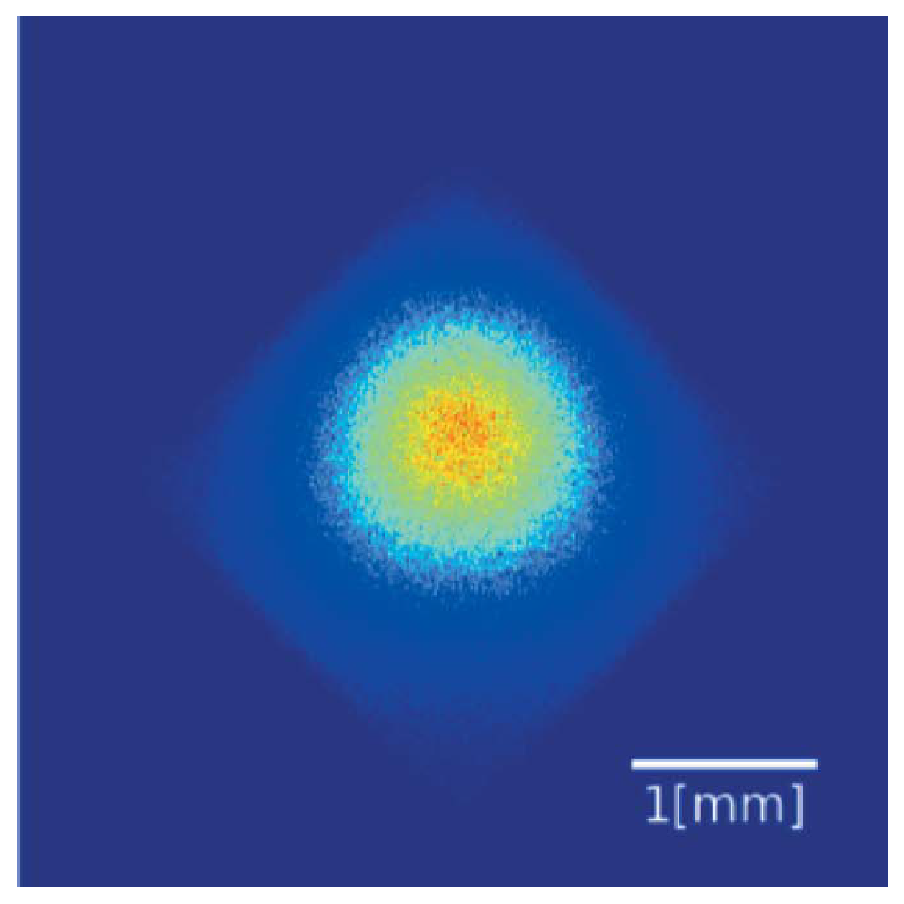
\includegraphics[width=.4\textwidth]{Immagini/Chapter5/PaperSpotMontel}}\quad
%
\subfloat[][Beam image divergence\label{fig: PaperImageDivergence}]
   {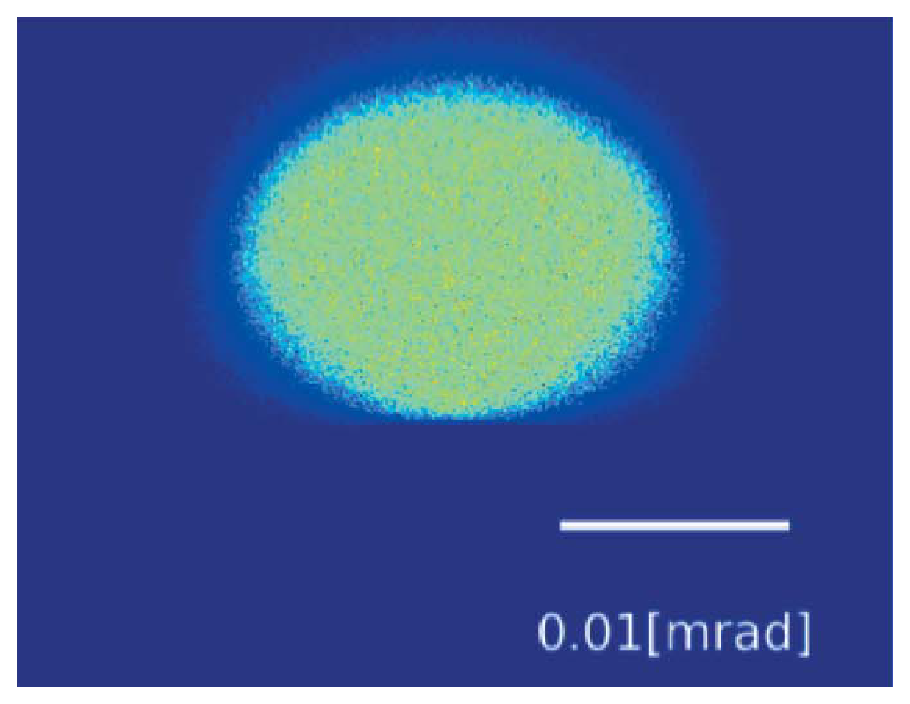
\includegraphics[width=.4\textwidth]{Immagini/Chapter5/PaperDivergenceMontel}}
%
\caption{Resuts of the Montel system of a source beam with a FWHM spot of 2.5$\mu $m and a Gaussian divergence of 5$mrad $}
%
\label{fig: PaperResults}
%
\end{figure}

\begin{figure}[H]
%
\centering
%
\subfloat[][Beam image shape\label{fig: Image dimension}]
   {\includegraphics[width=.48\textwidth]{Immagini/Chapter5/ImageDimension}}\quad
%
\subfloat[][Beam image divergence\label{fig: Divergence dimension}]
   {\includegraphics[width=.48\textwidth]{Immagini/Chapter5/DivergenceDimension}}
%
\caption{Results of  my Montel simulation of a source beam with a FWHM spot of 2.5$\mu $m and a Gaussian divergence of 5$mrad $}
%
\label{fig: My Simulation Comparison}
%
\end{figure}

\section{Analysis of Montel system}
To understand the Montel system is used the program defined, simulating different situation, studying the results obtained. To understand that Montel work well, it is simulated the behaviour of a pointwise source with a certain divergence, using a collimating system, and watching what happen to the beam. The  second step is to simulate a collimating beam with a certain source shape geometry and figure out the image plot obtained by a focalizing system in its image plane. What is expected is a point, in the velocity space for the first situation and in the real space for the second simulation, because this is the behaviour of an ideal collimating/focalizing system. For the simulation are used parabolical Montel and an incidence angle of 2$^{\circ} $ (the choice of the angle is arbitrary, that of the paraboic system is because is needed to collimate a beam, also for elliptical system is possible to tcollimate a beam using one focal distance very big).
\\
For the collimating system 


\section{Alignment}
Alignment of a beam is important for experimental use so, this section studies the behaviour of a beam when the beam is not perfectly align, in order to understand the behaviour of the beam in the different cases and act consequently. 
\\
The parameter that are changed are :
\begin{enumerate}
	\item orthogonality
	\item incidence angle
	\item point of incidence
\end{enumerate}
Using a focusing parabolic Montel system with a source of square shape having a side of 1$\mu $m, and a Gaussian divergence with FWHM of 25$\mu $m

\subsection{Orthogonality}
In this section is it done an orthogonality studies of the Montel system, it is studied the behaviour of a beam, using a source parameter defined before. Figure \ref{fig:HistogramFitted} presents the interesting histogram versus the horizontal angle $x^{'} $ when the angle between the mirrors change ($\alpha = 90^{\circ} + \Delta $). It can be noted a improvement of the collimation of the beam changing the angle in the case of closer mirrors ($\Delta = -0.004^{\circ} $).
\\
Figure show the trend of the FWHM of the $x^{'} $ changing the angle $\Delta $, it is possible to note a minimum for negative angle (this  situation correspond to the indigo line) after that the situation become worse. Moreover, the behaviour of the FWHM is not symmetric with respect to $0^{\circ} $, in case of negative angle deviation the situation improve for small range of deviation angle, after that, the trend get worse, on the opposite way, the situation get worse increasing the positive deviation angle. 

\begin{figure}
%
\centering
%
\includegraphics[width=.6\textwidth]{Immagini/Chapter5/HistogramFitted}
%
\caption{Nessuna immagine\dots Sorry.}
%
\label{fig:HistogramFitted}
%
\end{figure}

\begin{figure}
%
\centering
%
\includegraphics[width=.6\textwidth]{Immagini/Chapter5/FWHMChangingOrt}
%
\caption{Nessuna immagine\dots Sorry.}
%
\label{fig:FWHM changing orthogonality}
%
\end{figure}
\subsection{Incidence angle}
\subsection{point of incidence}
Another way that can be studied to align correctly a beam, is to study the behaviour of a non centred beam with respect to the center of the Montel system. In this section is reported the behaviour about the change of FWHM of both $x^{'} $ and $z^{'} $ following different path. Figure \ref{fig: path} show the different path followed to simulate the non-centred beam that are named:
\begin{enumerate}
	\item Y
	\item XZ
	\item XYZ1
	\item XZY2
\end{enumerate}

\begin{figure}[H]
%
\centering
%
\includegraphics[width=1.\textwidth]{Immagini/Chapter5/Cattura2}
%
\caption{Different path for simulate the non-centred beam}
%
\label{fig: path}
%
\end{figure}

Figure \ref{fig: reuslt diff. path} show the behaviour of the two FWHM of the beam changing the incidence point of the beam moving the different paths. This point is defined with respect to the center of the Montel system that correspond to the origin (0, 0, 0). In Figure \ref{fig: Y path}, the incidence point move along y-axis, start from the point (0, 1.5mm, 0) and arriving to the point (0, -1.5mm, 0), and show, more or less, a flat behaviour of the FWHM. Figure \ref{fig: XZ path} start from the point (0, 0, 0.15mm) and arrive to (-0.15mm, 0, 0) and have specular behaviour for the two FWHM, there is a minumum of the two FWHM near the origin point, moving on the oe1 worse the FWHM of $z^{'} $ and maintain the other constant, on the contrary, moving on the oe2 the situation is reversed, in this case the FWHM of $x^{'} $ get worse, maintaining constant the one of $z^{'} $. Figure \ref{fig: XYZ1 path} start from (0, 1.5mm, 0.15mm) and arrive to (-0.15mm, -1.5mm, 0) and Figure \ref{fig: XYZ2 path} start from (-0.15mm, 1.5mm, 0) and arrive to (0., -1.5mm, 0.15mm). The behaviour of this last two path are similar to that of \ref{fig: XZ path}, this is reasonable, because the motion along y-axis does not influence the FWHM because of the definition of the cylindrical mirror, that in any point along the y direction have the same geometry.


\begin{figure}[H]
%
\centering
%
\subfloat[][Y path\label{fig: Y path}]
   {\includegraphics[width=.4\textwidth]{Immagini/Chapter5/Ypath}}
%
\subfloat[][XZ path\label{fig: XZ path}]
   {\includegraphics[width=.4\textwidth]{Immagini/Chapter5/XZpath}}\quad
%
\subfloat[][XYZ1 path\label{fig: XYZ1 path}]
   {\includegraphics[width=.4\textwidth]{Immagini/Chapter5/XYZ1Path}}
%
\subfloat[][XYZ2 path\label{fig: XYZ2 path}]
   {\includegraphics[width=.4\textwidth]{Immagini/Chapter5/XYZ2Path}}
\caption{Resuts of the Montel system of a source beam with a FWHM spot of 2.5$\mu $m and a Gaussian divergence of 5$mrad $}
%
\label{fig: reuslt diff. path}
%
\end{figure}

